´%%==========================
%% chapter01.tex for TJU Master Thesis
%% based on CASthesis
%% modified by charlie.yaha@gmail.com
%% version: 0.1alpha
%% Encoding: UTF-8
%% last update: Dec 5th, 2010
%%==================================================

%\bibliographystyle{TJU} %[此处用于每章都生产参考文献]


\chapter{绪~论}
\label{chap:introduintroduction}
\section{研究背景}



液压系统是航空航天等产品的重要系统。而液压系统的各类管线,是现代航空航天工业中极为重要的部件,对其可靠性的要求仅次于发动机。

现代飞机航面操纵系统与动力收放系统几乎都是液压驱动的。液压系统作为飞机飞行控制系统和起落架等负载的动力源,对飞机的安全飞行起着关键的作用。
大型客机的液压系统,是一个多余度、大功率的复杂综合系统,控制着飞机起落架、襟翼、减速板的收放,平尾、副翼、方向舵的操纵,进气锥、辅助进气门的调节等\cite{dingfei2010}。空客的A320,波音的B737都配备了至少3套相互独立的液压\cite{dingfei2010},多套液压系统相互独立、相互备份,管线密布机身,如图\ref{fig:plane-hose}所示,管线长度一般在机身长度的数倍以上。


\begin{figure}[!htbp]
	\centering
	%	\subfigure[起落架]{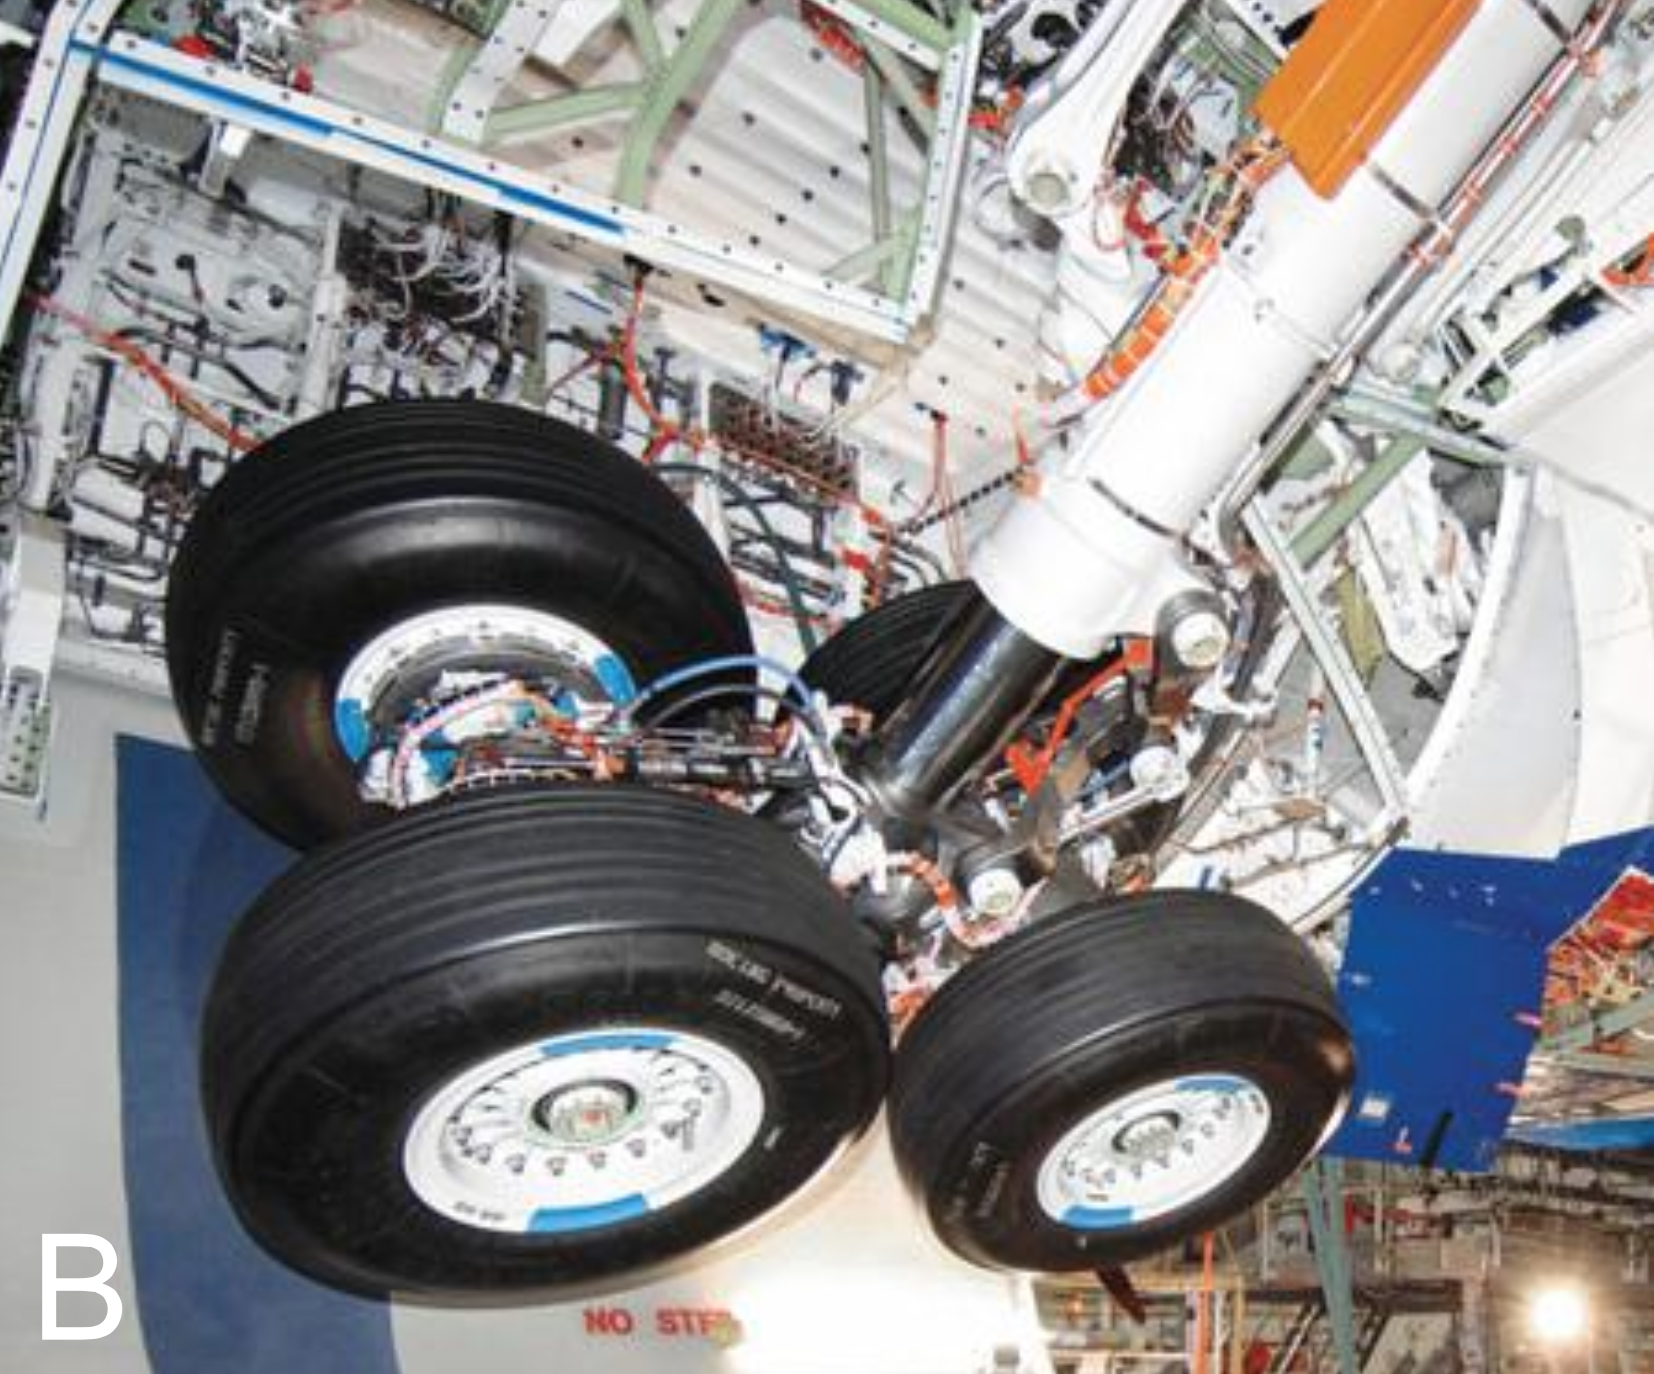
\includegraphics[width=0.4\textwidth]{figure/chap1/gear}}		\label{fig:plane gear}
	%	\hspace{1cm}
	%	\subfigure[飞机管路]{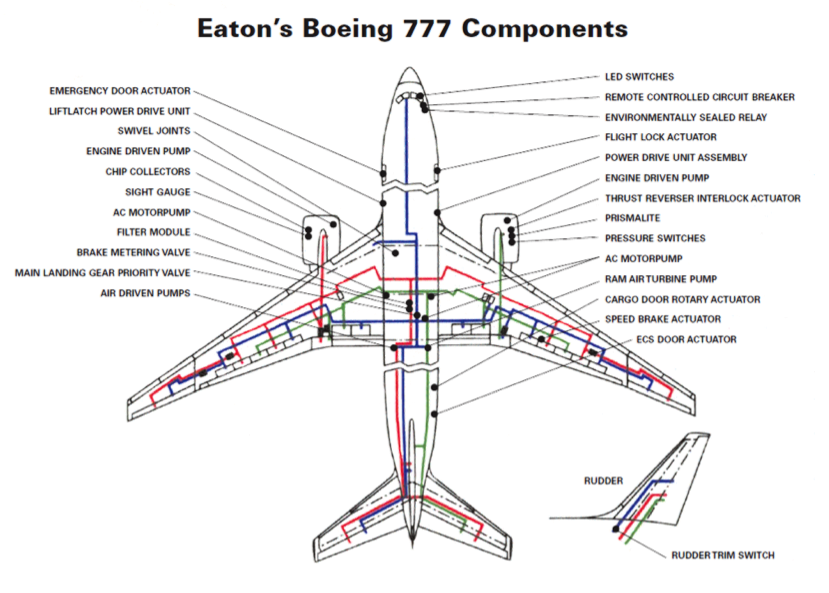
\includegraphics[width=0.5\textwidth]{figure/chap1/Plane}}    \label{fig:plane}
	\subfigure[机身软管管路(a.软管,b.液压源)]{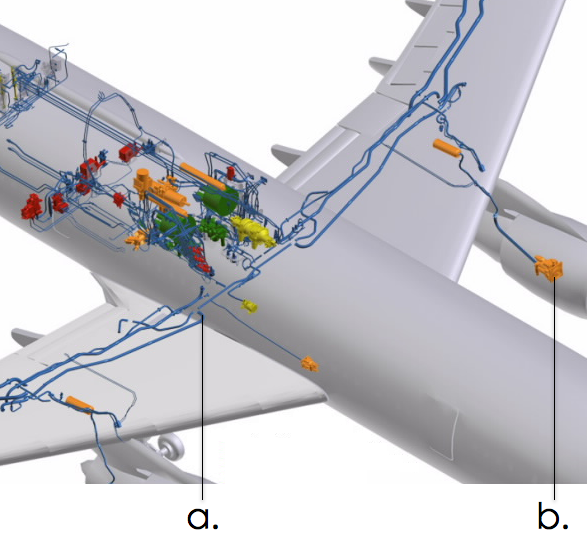
\includegraphics[width=0.4\textwidth]{figure/chap1/plane-cruit}\label{fig:plane-cruit}}    
	\hspace{1cm}
	\subfigure[发动机软管管路(a.软管,b.液压源)]{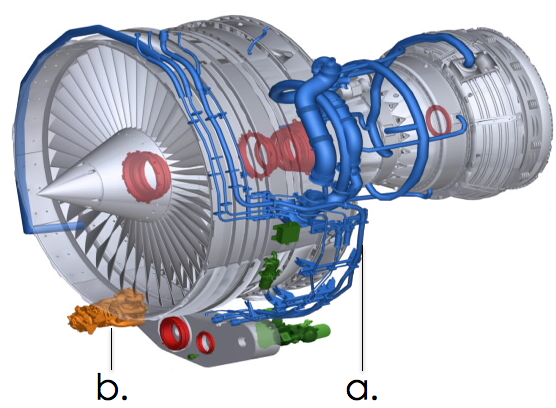
\includegraphics[width=0.4\textwidth]{figure/chap1/engine-cruit}\label{fig:engine-cruit}}    
	\bicaption[fig:Distribution of hose assembly]{飞行器液压系统管线分布}{飞行器液压系统管线分布}{Fig}{Distribution of hose assembly in a plane}  
	\label{fig:plane-hose}
\end{figure}



据统计,当前我国飞机液压系统的故障几乎都发生在管路部分,
而液压系统的故障约占飞机机械系统总故障的左右$1/3 $,飞机液压系统的维修工作量占机械维修工作量的$ 30\%$\cite{lijun2007},
液压软管的可靠性问题是飞机故障、事故的主要原因之一。

液压管路的泄漏、失效往往是由液压泵的压力脉动引起的。现代飞机液压系统大多采用变量柱塞泵,脉动式的流量输出是其固有特性;同时液压系统工作时,在阀门打开或关闭的瞬间,供压管路和回油管路会出现强烈的压力撞击,即压力脉冲。变量柱塞泵产生的压力脉动,在高速、高压、高温、大流量条件下,若与系统匹配不当,油泵出口压力会产生高频等幅振荡,从而很容易导致两种耦合振动:一种是脉动频率与流体谐振频率接近时的耦合振动;另一种是脉动频率与管路系统结构的固有频率接近时,发生的耦合振动。
在高压管路上,压力脉冲峰值有可能达到系统额定压力的1.5倍以上,而在回油管路上则可能达到正常回油压力值的10倍以上\cite{lijun2007}。
这种脉冲峰值很容易导致管壁破裂、管路支撑结构破坏,引起支撑刚度下降、管路系统失效、液压油液泄露,从而导致严重的灾难性事故\cite{gaofeng2013}。


例如,我国七十年代研制的某机型,从油泵出口至蓄压器之间的软管管路不断发生断裂,影响到设计定型;
八十年代初,我国研制的某型号机地面试车时,由于液压软管爆裂引发大火,致使整架飞机毁于一旦,不仅造成巨大的经济损失,而且使型号研制进度推迟了两年;某型机的泵出口软管出现多次爆裂事故,由于管路断裂,液压系统失效,发生了飞机启用应急系统、强迫着陆及驾驶员应急跳伞等严重问题\cite{lijun2007,guoqing2010,gaofeng2013}。

\begin{figure}
	\centering
	\subfigure[波音b777起落架液压软管]{
		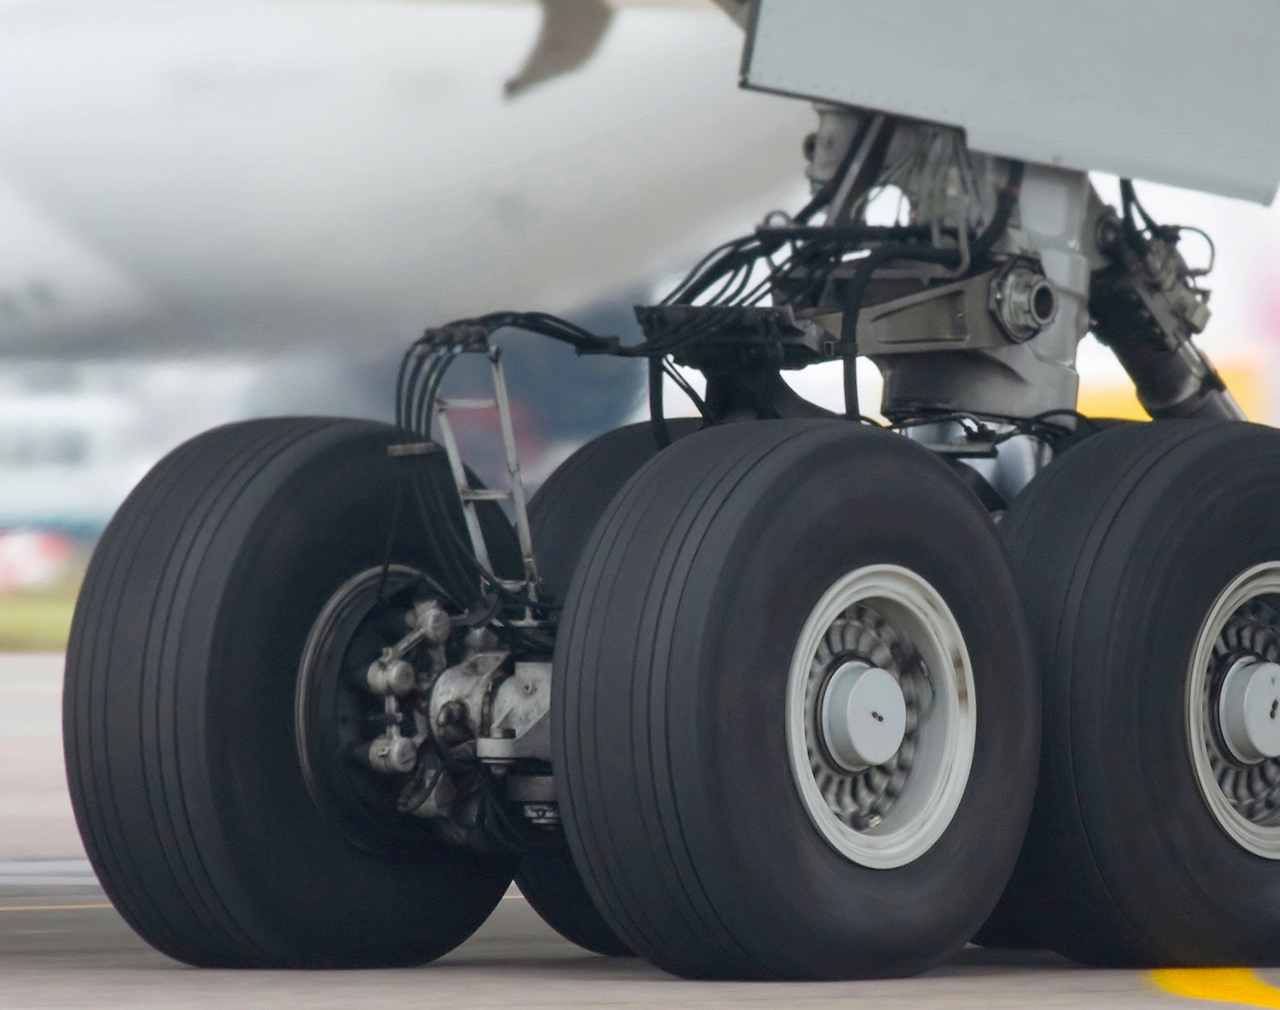
\includegraphics[width=0.4\textwidth]{figure/chap1/777-gear}\label{fig:777-gear}}
	\hspace{1cm}
	\subfigure[a380起落架液压软管]{
		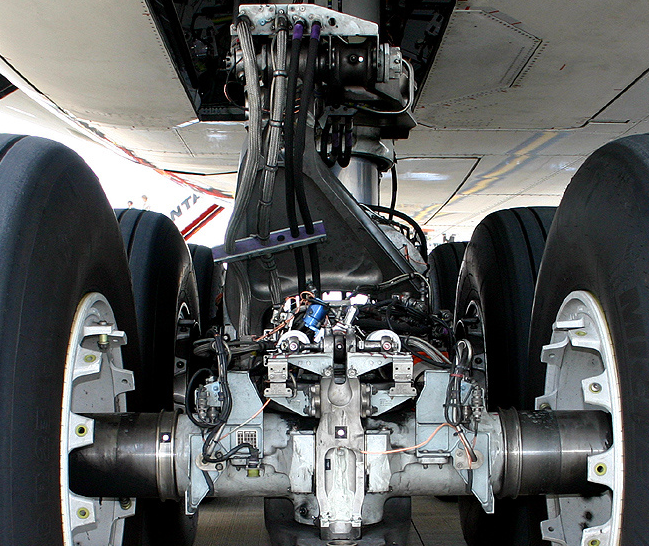
\includegraphics[width=0.4\textwidth]{figure/chap1/a380-gear}\label{fig:a380-gear}}
	\bicaption[fig:gear hose cruit]{起落架软管管路}{起落架软管管路}{Fig}{Hydraulic hose cruit of gear}  
	\label{fig:plane-hose}
\end{figure}



因为液压泵出口处的高频振动,刚性管受激共振而破坏失效,必须要低刚度的柔性管来吸收振动的能量,
同时因为飞机液压能源系统由于飞机对空间和质量的限制,常常具有一般管路设计中需要避免的长跨度、低刚度管段出现\cite{gaofeng2013}。
因此,飞机动作控制液压系统(\ref{fig:plane-cruit})以及飞机引擎液压、燃油系统(\ref{fig:engine-cruit})中,大量的管道并非刚性管,而是由大量柔性软管组成的。


随着航空技术的不断发展,飞机液压系统也在向高压化、大功率的方向发展。
因为提高飞机的液压系统工作压力是减小系统自身重量和体积的重要手段。
空客A320液压系统额定工作压力为3000psi(21MPa)
最新的客机型号波音的B787和空客A380的的液压系统压力等级都达到 5000psi(35MPa)\cite{lavooij1991},
国外领先企业Eaton Aerospace、Parker Hannfin公司也已经为军用飞机开发出来8000psi(55MPa)的液压泵,空客公司也已经提出了将起落架刹车制动液压管路工作压力提高到8000psi(55MPa)的目标,而国内的液压系统一般只能做到3000psi(21MPa)。


\begin{figure}
	\centering
	\subfigure[软管失效]{
		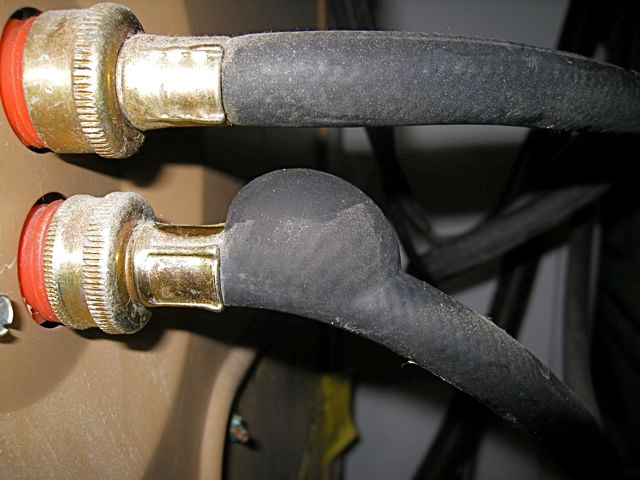
\includegraphics[width=0.3\textwidth]{figure/chap1/burst-hose-1}}
	\hspace{1cm}
	\subfigure[软管失效]{
		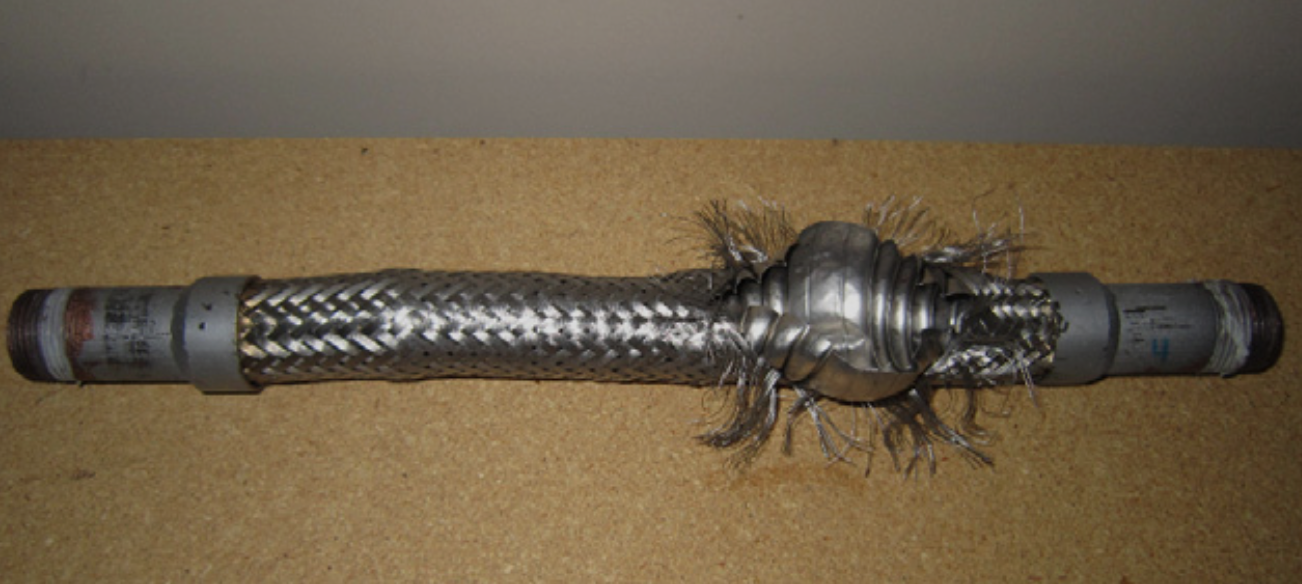
\includegraphics[width=0.5\textwidth]{figure/chap1/burst-hose-2}}
	\bicaption[fig:hose burst]{软管失效}{软管失效}{Fig}{hose fail}  
	\label{fig:plane-hose}
\end{figure}





液压泵脉动控制方面,国内液压泵一般流量脉动为$\pm10\%$,国外一般在$ \pm5\% $左右\cite{lijun2007}。Eaton公司为空客A380最新研制出一种内置衰减器的柱塞泵,压力脉动变化为$ \pm 1\%$。可见国内液压泵脉动控制的水平距国际先进水平尚有一定距离,考虑到新型柱塞泵的研发周期,这种差距短期之内很难弥补。
而飞机液压系统的压力脉冲是造成液压管路提前损坏,导致液压系统故障的主要原因之一。这就对我国液压管路的设计、生产水平提出了更高的要求。





%了解什么事软管
\section{软管组件简介}
%软管定义,软管组件结构

在因为在实际工程环境中,特别是各类飞行器中,很多情况下刚性管无法使用,例如:1)液压元件持续的运动,2)液压元件任意或不规则排列,3)安装空间不足
4)管路剧烈振动,
5)管路受到冲击,
6)管路区段有高压力的释放。
为了克服以上不利条件,一般采用柔性的液压软管。这种柔性液压软管是一种复合结构的管路连接件,一般将整个系统结构称为软管组件(Flexible Hose Assembly),或软管总成(本文统一称为软管组件)。





其结构包括了柔性内管、加强层、保护层,以及金属连接件。
柔性软管的材料一般为橡胶管,氟塑料管,热塑料管,金属波纹管等;内管外包覆若干层加强结构,如编织、缠绕等。
软管组件工作时,绝大部分内压荷载由加强层承担,内管主要起通道的作用。加强层数一般视内压荷载大小而定。


\begin{figure}[!htbp]
	\centering
	\subfigure{
		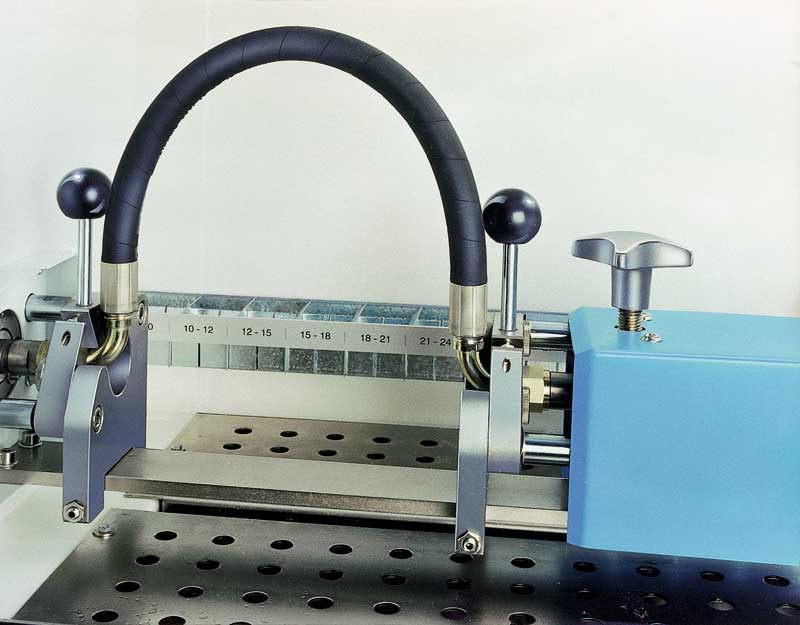
\includegraphics[width=0.45\textwidth]{figure/chap1/hose1}}
	\hspace{0.5cm}
	\subfigure{
		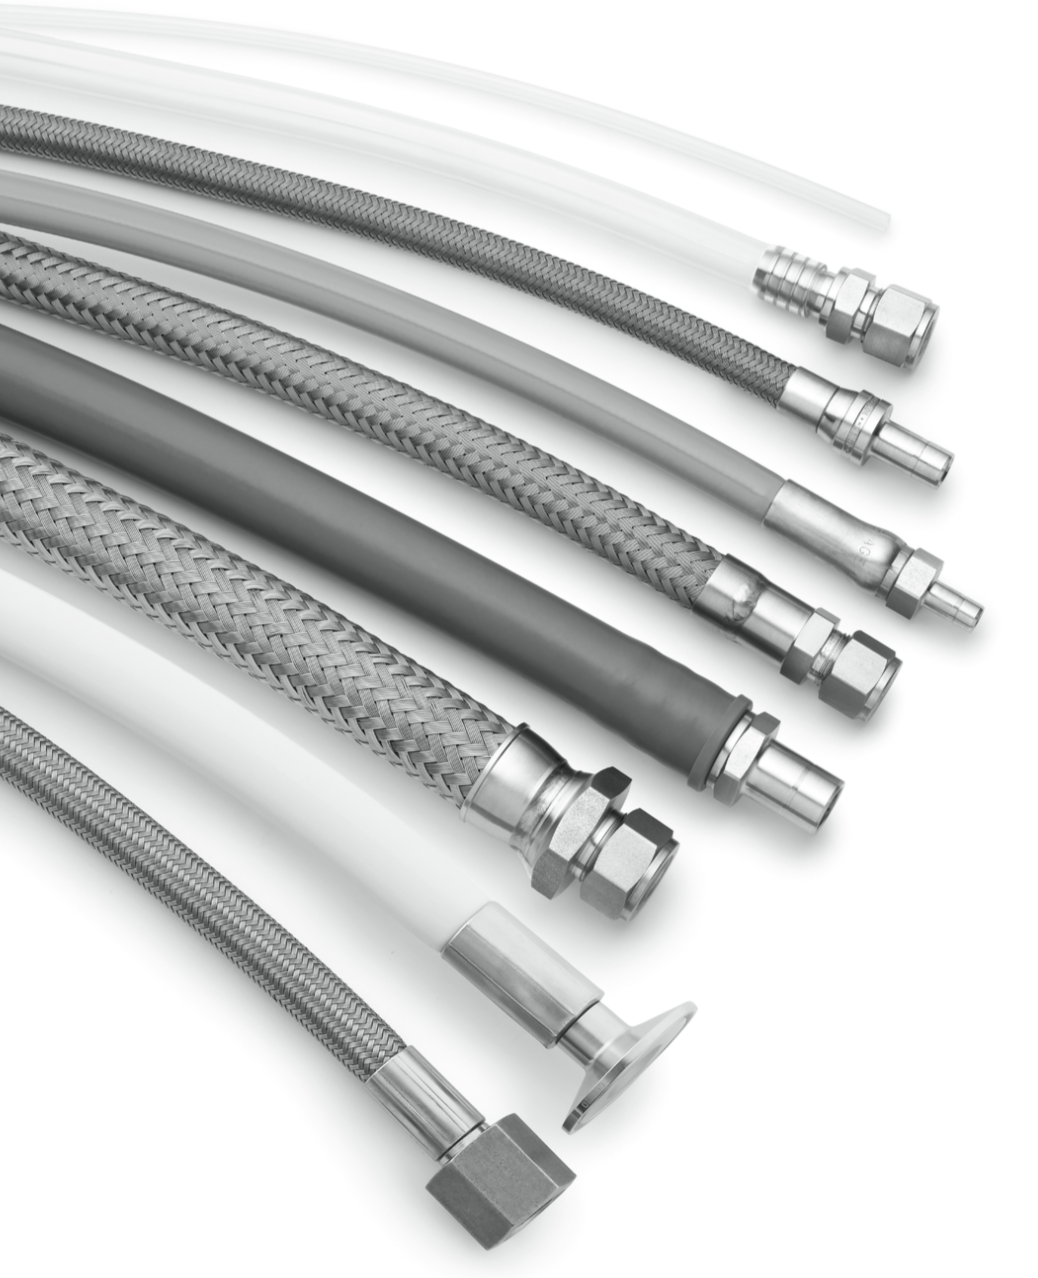
\includegraphics[width=0.3\textwidth]{figure/chap1/hose2}}
	\bicaption[fig:hose burst]{软管组件}{软管组件}{Fig}{Hose Assembly}  
	\label{fig:hose}
\end{figure}


软管组件同时也应用于气动、燃油、滑油等系统的介质传输,起到了“血管”作用,航空航天飞行器、汽车、船舶,以及各种工业设备、机床等,都大量使用了软管组件。相比普通硬质管,软管组件可以承受相对较大的内压、轴向荷载,同时保持较小的质量、弯曲刚度,带来以下优势:可以减小系统的刚度,吸收液压源产生的振动;安装方式灵活,节约了系统内部的空间。




%软管优势



%不同软管型号
软管组件根据不同的压力等级可以分为低压、中压、高压、超高压几种型号,如表\ref{tab:hosepressurelevle}所示,


\begin{table}[!htbp]
	\centering
	\bicaption[tab:hosepressurelevle]{软管组价压力等级}{软管组价压力等级}{Table}{Hose Assembly Pressure level}
	\label{tab:hosepressurelevle}
	\begin{tabular}{ccc}
		\toprule
		    &   英制    &  公制  \\ \midrule
		低压  & $ \le$1000psi  & $ \le$7MPa \\
		中压  &  1000psi   \textasciitilde  3000psi  & 7MPa   \textasciitilde  21MPa \\
		高压  &  3000psi   \textasciitilde  4000psi &  21MPa   \textasciitilde  28MPa\\
		超高压 & $ \ge$4000psi &  $ \ge$28MPa  \\ \bottomrule
	\end{tabular} 
\end{table}

根据美国\footnote{SAE AS1946,SAE AS604,SAE AS1339}、欧洲以及国际标准化组织\footnote{ISO1436,ISO3862
}的安全标准,软管组件的脉冲安全系数为$ 4:1 $,
即软管组件受压力脉冲破裂时,所使用的真实压力需达到4倍额定压力,一般将该压力值定义软管组件的爆破压力。
因此,低压软管的爆破压力一般在以下30MPa;目前国内3000psi液压系统配套的软管组件,其爆破压力至少为85MPa;国际新一代大型客机已经要求软管组件爆破压力至少为140MPa。


根据软管组件内管管径的不同,可以分为轻型、中型、重型,
管径在6mm以下的一般归为轻型管,管径14mm以上的为重型管。

根据不同的工作压力、流量的需求,各型软管的常见用途如表\ref{tab:hosefixposition}所示,

\begin{table}[!htbp]
	\centering
	\bicaption[tab:hosefixposition]{不同型号软管组件安装位置}{不同型号软管组件安装位置}{Table}{Position}
		
	\begin{tabular}{ccc}
		\toprule
		&    轻型     &     重型     \\ \hline
		低压 & 汽车刹车、转向传动 &  输运水、气  \\
		高压 & 飞机起落架、襟翼  & 飞机、船舶液压泵出口 \\ 
		\bottomrule
	\end{tabular} 
\end{table}

%解释表格
飞机、船舶液压泵出口处压强高,流量大,震动强,工作环境极为恶劣,因此国内外一般都采用重型高压软管组件,技术也都较为成熟。
飞机起落架、襟翼等部位处于机身液压系统的末端,但压强仍然很高,而且软管的安装空间很小,要求软管组件具有较小的弯曲半径。保持较高的爆破压力的同时,使得软管组件小型化、轻型化,这就对软管组件的设计水平提出了很高的要求。国外企业在轻型高压软管组件领域技术优势明显,基本垄断了该市场。
以飞机液压系统高压化的趋势,我国在这一领域的短板会更加明显的凸显出来。而这一型的软管组件,仅仅依靠看经验防止已经很难实现,对科学可靠的设计理论的探求已迫在眉睫。

汽车领域也大量使用了软管组件,例如刹车制动管,转向传动管,空调管等。相比飞行器的液压系统,汽车的液压系统压强较低,如刹车制动管的爆破压力一般为35MPa至40MPa\footnote{GB 16897-2010}。但汽车行业对成本较为敏感,要求在保证设计指标的同时,使软管的结构达到最优化。这对软管的设计、制造也提出了很高的要求。

 	 	 
					
\section{软管组件行业现状}
\label{chap:hose-generation}

软管组件的加工生产技术经过几次重大变革,至今为止,已经发展出了3代产品。
金属增强软管组件是由美国发明并于上世纪60年代开始用于飞机的液压系统,
%第一代
在此之前为第一代软管组件,以橡胶软管为主;

从上世纪60年代到上世纪90年代中期,
第二代金属加强软管已经广泛应用于航空、航天领域。同时也根据不同的压力等级需求和工作环境发展出不同的加强形式,如编织加强、缠绕加强;也发展出了不同的内管材料,如PTFE氟塑料、热塑料、尼龙等;还出现了防火、防磨损、防腐蚀、防紫外线等各式附件,品种繁多。
为此,美国建立了一系列的军用、宇航产品技术标准或规范,例如:MIL-H-25579E、SAE AS604、SAE AS614等。
第二代软管组件的最高使用温度已达232\textcelsius,最高工作压力已经达55MPa。
已经广泛应用于各种类型的飞机和导弹、运载火箭等,例如:F-16、F-22、波音客机等。


%第三代
近年来,航空航天事业飞速发展,对软管组件也提出轻量化的要求,传统钢丝增强软管组件已不能满足航空航天的设计要求。
为了解决这个问题,美国Titeflex、Eaton及Parker等国际知名公司,已在20世纪80年代,开始了非金属增强软管组件的研究,也就是第三代软管组件。他们纷纷研制推出了各自的非金属增强软管组件产品。目前波音B787就大量使用了Eaton公司的AS1975以及AS4623 Kevlar加强软管组件,满足5000psi(35MPa)工作压力要求。

\begin{figure}[!htbp]
	\centering
	\subfigure{
		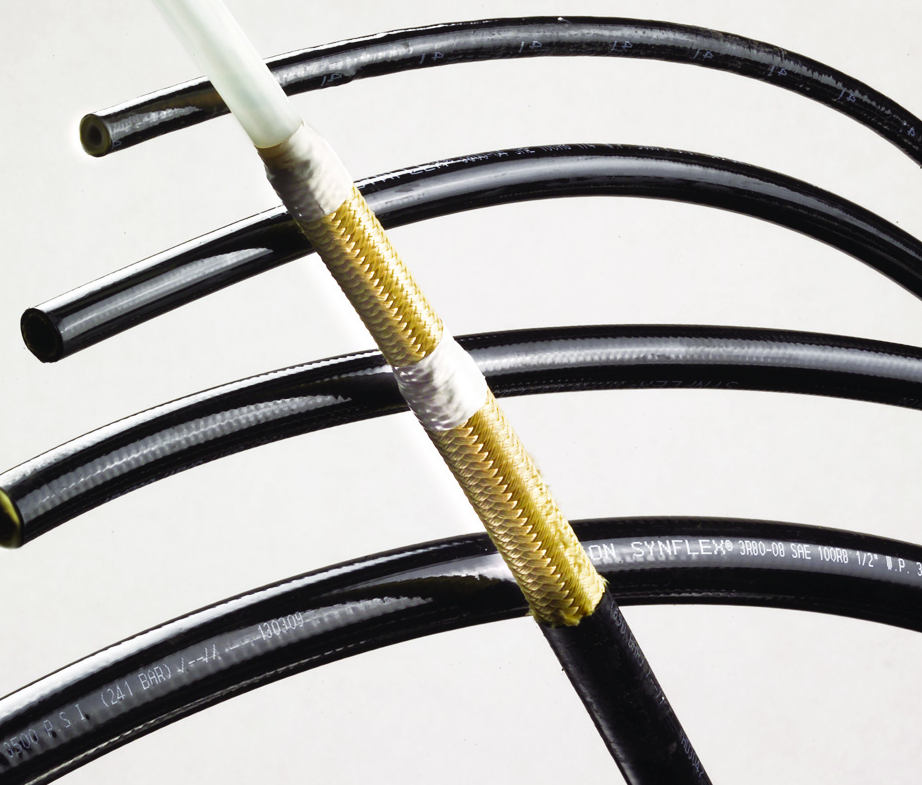
\includegraphics[width=0.3\textwidth]{figure/chap1/kevlar-hose}}
	\hspace{0.5cm}
	\subfigure{
		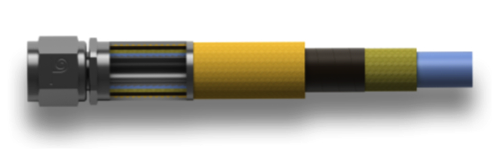
\includegraphics[width=0.5\textwidth]{figure/chap1/kevlar-hose-2}}
	\bicaption[fig:kevlar-hose]{Kevlar加强软管组件}{Kevlar加强软管组件}{Fig}{Kevlar Reinforced Hose Assembly}  
	\label{fig:kevlarhose}
\end{figure}


我国目前钢丝增强液压软管年产量约6000万米\cite{xuhaitao2013},但大多为低端低压产品。
尚未出现非金属纤维增强的软管组件,都属于第二代金属纤维增强的范畴。相对较为先进的国产软管组件也只达到了5000psi(35MPa)。并且国内尚无航空软管的相应标准,没有有成熟的规范、标准试验设施和完整的试验方法。可以说国内软高端管组件行业还处于起步阶段,距离轻量化,标准化,高压化的国际水平还有不小的距离。

\section{软管组件研究现状}
针对软管组件的研究有两个方向:1)加强层的力学行为和力学本构;2)连接件与管体的扣压工艺过程。

软管组件的理论研究始于20世纪50年代,理论体系源于螺旋钢绞线(Helical Strands)。螺旋钢绞线这种结构主要用于大桥的悬索和输电线的加强。
\begin{figure}[!htbp]
	\centering
	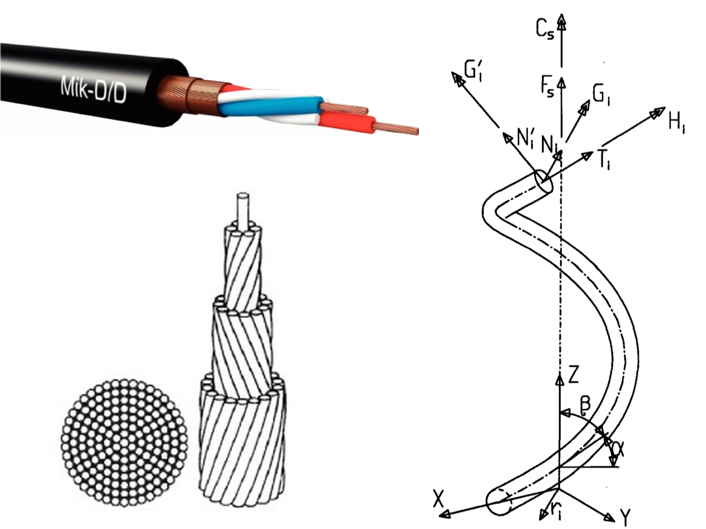
\includegraphics[width=0.6\textwidth]{figure/chap1/helical-strands}
	\bicaption[fig:hose burst]{软管组件}{软管组件}{Fig}{Hose Assembly}  
	\label{fig:hose}
\end{figure}
螺旋钢绞线中的钢丝纤维直径一般较大,因而不能忽略钢丝的扭转刚度。
在这种理论体系下,讨论钢丝加强层的力学性能时,往往更加关注钢丝本身的力学行为。这种钢绞线结构(Helical wound assembly)由于结构的复杂性,形成了一套独特的基于实验和经验的理论体系\cite{Cardou1997}。虽然有学者尝试用弹性力学推导理论解\cite{phillips1972,machida1973},但主要仍以经验公式为主。

软管组件的加强层一般采用较细的钢丝,比较类似于复合材料中的纤维,仅在金属丝轴向可以承受拉伸荷载。但是当时符合材料力学并未充分发展,因而软管组件沿用了螺旋钢绞线的理论,主要研究缠绕的加强方式\cite{Entwistle1977,Knapp1979},将编制作为一种特殊的缠绕方式来研究\cite{Breig1988}

传统的编织和缠绕理论是将各层编织角和缠绕角均设计为 ,
这个角度是从通过柱状薄壁容器理论推导得出的,使得单层金属缠绕液压软管轴向和环向受力平衡。
但是对于多层加强软管组件,这种中性角度下钢丝在受内压时变形较大、钢丝间应力损失大\cite{Evans2002},不能发挥每根钢丝的最大强度,但对像高压胶管这种多层增强的厚壁管体,这个角度就很不适用了。比如按这个角度设计的胶管,一个工作层其爆破压力可达理论值的80\%纬左右,两个工作层约75\%,三个工作层只有65\%左右,四个工作层或小口径的三个工作层,要达到50\%都有一定困难。各增强层受力不均,内层应力大,外层应力小,且逐层递减。在脉冲试验和实际使用中,内层钢丝常因疲劳而断裂,中层和外层却完好无损,严重影响;对于编制加强软管组件,钢丝之间的相互影响更为复杂,传统的编织平衡角理论不能很好地反映出这种区别。

近年来,有文献研究了多层钢丝增强软管内压、应力与变形的综合的动态平衡体系[7],介绍了最佳角度数列的计算方法,但是没有用严格的数学方法来推导出各层钢丝的最佳角度值。因此利用计算仿真软件来分析各层钢丝角度的组合形式对软管受力的影响是一种有效的方法[8]。 

在连接件扣压的方向,早期研究较为少见,近年来,随着数值仿真手段的发展,学者也对液压软管总成连接质量的影响因素进行了研究,分析了扣压工艺、接头形式如芯子和外套的结构等因素对软管总成连接质量的影响。建立了分析模型,分析了扣压力、扣压量的大小对软管总成连接质量间的关系,并对扣压过程进行了控制。

具体的发展过程在第二章中有详尽的阐述。


\section{研究意义}

科技战略价值:大飞机,国产化。

研究价值:编织理论。

\section{研究主要内容}
本可以以软管组件为研究对象,围绕纤维加强层的力学本构的问题,分析了其非线性段的力学行为的结构机理,形成了一套分析方法和
本文主要的研究内容有:
\begin{asparaenum}
	\item 针对软管组件进行了拉伸试验,结合已有的理论,找到了实验中需要关注、记录的关键参数,并针对这些参数,分别设计了测量记录参数的方案。
	\item 根据实验结果与现有理论不吻合的部分,分析了可能导致这种差别的原因,排除了实验误差,挖掘出现有理论提升的空间。
	\item 参考符合材料力学处理编织问题的方法,提出了一套可以解释实验中出现的非线性段力学行为的理论,修正了编织层的刚度,分析讨论理论中各个参数的意义。
	 \item 
	利用准静态的分析方法对软管爆破试验进行了分析,建立了一套可以表针编织层强度的理论。
\end{asparaenum}

 
